\documentclass[times, utf8, proizvoljni, numeric]{fer}

\usepackage{booktabs}
\usepackage{amsmath}
\usepackage{nccmath}
%\usepackage{hyperref}
\usepackage[section]{placeins}
\usepackage{indentfirst}

\usepackage{footnote}
\usepackage{graphicx}
\usepackage{float}
\usepackage{mathtools}
\usepackage{makecell}
\usepackage[hidelinks]{hyperref}

\renewcommand\theadalign{cb}
\renewcommand\theadfont{\bfseries}
\renewcommand\theadgape{\Gape[4pt]}
\renewcommand\cellgape{\Gape[4pt]}

\DeclarePairedDelimiter\ceil{\lceil}{\rceil}
\DeclarePairedDelimiter\floor{\lfloor}{\rfloor}

\DeclareMathOperator*{\argmin}{\arg\!\min}
\DeclareMathOperator*{\argmax}{\arg\!\max}
\begin{document}


\title{Ekstrahiranje značajki slika pomoću dubokog učenja u svrhu poboljšanja sustava preporuke slika}
\author{Toni Vlaić, Viran Ribić}

\maketitle

% Ispis stranice s napomenom o umetanju izvornika rada. Uklonite naredbu \izvornik ako želite izbaciti tu stranicu.
% Dodavanje zahvale ili prazne stranice. Ako ne želite dodati zahvalu, naredbu ostavite radi prazne stranice.
\thispagestyle{empty}
\zahvala{\begin{center}Ovaj rad izrađen je u Zavodu za elektroniku, mikroelektroniku, računalne i inteligentne sustave Fakulteta elektrotehnike i računarstva Sveučilišta u Zagrebu pod vodstvom doc. dr. sc. Marina Šilića i predan je na natječaj za dodjelu Rektorove nagrade u akademskoj godini 2017./2018.
		\end{center}
}

\tableofcontents
\thispagestyle{empty}
\listoftables
\thispagestyle{empty}
\listoffigures
\thispagestyle{empty}
%%%%%%%%%%%%%%%%%%%%%%%%%%%%%%%%%%%%%%%%%%%%%%%%%%%%%%%%%%%%%%%%%%%%%%%%%%%%%%%%%%%%%%%
%% CHAPTER
\chapter{Uvod}


\section{Opći i specifični ciljevi rada}

Hipoteza ovog istraživanja bila je da se korištenjem dubokog učenja može razviti sustav koji uspješno stvara nisko dimenzionalne reprezentacije slika proizvoljnih veličina kako bi se iste mogle efikasnije grupirati i pretraživati po njihovim semantičkim značajkama te iskoristiti u sustavima za preporučivanje temeljenim na sadržaju ili kao dodatak sustavima preporuke temeljenim na kolaborativnom filtriranju.

Cilj ovog istraživanja bila je ostvariti takav duboki model te ispitati različite načine ekstrakcije značajki iz dubokih modela te metrika kojima se ekstrahirane značajke mogu uspoređivati. Također za kraj potrebno je i razviti prototip jednostavnog sustava za preporučivanje temeljen na sadržaju koji koristi značajke ekstrahirane razvijenim modelom.

\section{Programska i hardverska podrška}
\subsection{Programska podrška}
\noindent Python \\
Tensorflow - u literaturi ti linkah rad pa mos nesto citirat cisto za reference dok ovo budes opisivao \cite{tensorflow2015-whitepaper}\\
OpenCV - preprocessing i loadanje slikica (to mogu ja slozit) \cite{itseez2015opencv}\\
NMSLIB - brza pretraga skalabilnost etc (ono sta napisah u literaturi isto) \cite{NMSLIB}\\
TSNE - za vizualizaciju (to mogu ja opisat) \cite{TSNE}\\
Django?\\

\subsection{Hardverska podrška}
Implementacija rješenja i ispitivanje napravljeno je na računalu s operativnim sustavom Ubuntu 16.04. Od važnijih komponenti koje utječu na brzinu i mogućnost reprodukcije rezultata bitno je naglasiti da računalo ima grafičku karticu GTX Titan Pascal s 12GB memorije, intelov i7 procesor sa šest jezgri i 32GB radne memorije što je omogućilo obradu velikog podatkovnog skupa u razumnom vremenu

%%%%%%%%%%%%%%%%%%%%%%%%%%%%%%%%%%%%%%%%%%%%%%%%%%%%%%%%%%%%%%%%%%%%%%%%%%%%%%%%%%%%%%%
%% CHAPTER
\chapter{Modeli za sažimanje}

\section{Konvolucijske mreže}

Konvolucijske neuronske mreže su postale popularne kao sredstvo za obradu slika nakon pobjede Alexa Krizhevsky-og na natjecanju 2012 ILSVRC (ImageNet Large-Scale Visual Recognition Challenge \cite{ILSVRC15}) sa svojom konvolucijskom neuronskom mrežom danas poznatijom pod imenom AlexNet. Od tada je njihova popularnost kao sredstvo za obradu slika naglo porasla te su danas konvolucijske arhitekture najdominantnije na području obrade slika.

Računalo promatra sliku kao trodimenzionalnu matricu dimenzija X*Y*Z gdje se dimenzija Z može smatrati brojem kanala promatrane slike (uobičajeno crveni-zeleni-plavi kanal, poznatije kao RGB). Uzimajući u obzir da su ulazni podaci modela konvolucijske mreže uobičajeno slike, odnosno trodimenzionalne matrice, ona svoje neurone kojima obrađuje primljene podatke također uređuje u tri dimenzije širina, visina i dubina koja se može smatrati i brojem kanala kao u slikama, no bez limitacija na broj istih.

Jedna duboka konvolucijska mreža se uobičajeno gradi od konvolucijskih slojeva, slojeva sažimanja i potpuno povezanih slojeva unaprijedne neuronske mreže. Između svih slojeva u mreži nalazi se tzv. aktivacijska funkcija čiji je cilj uvesti nelinearnost u model.

Aktivacijske funkcije su hiperparametri svake mreže i bitne su zbog unošenja nelinearnosti inače bi se mreža reducirala na afinu transformaciju koja preslikava ulazne vrijednosti u izlazne. Aktivacijska funkcija završnog sloja ovisi o tipu zadatka koji se mreža uči rješavati. Mreža trenirana za aproksimaciju funkcije neće raditi transformacije nad izlazom, već će aktivacijska funkcija izlaza biti funkcija identiteta. Drugi primjer bio bi zadatak klasifikacije za koji izlaz mora imati probabilističku interpretaciju, a ona se postiže sigmoidom u slučaju dvije klase ili softmax funkcijom za više klasa. 


\subsection{Konvolucijski slojevi}

Konvolucijski sloj odrađuje većinu posla u konvolucijskoj mreži. Novost u konvolucijskoj mreži je povezivanje svakog neurona s malom regijom prethodnog sloja umjesto potpunog povezivanja svih neurona između slojeva kao u potpuno povezanoj unaprijednoj mreži. Svaki konvolucijski sloj ima tri dimenzije i neuroni svakog kanala dijele filtere s kojima računaju izlaze iz prethodnog sloja.

Uzmimo za primjer jedan konvolucijski sloj koji obrađuje CIFAR (\cite{CIFAR10}) skup podataka s dimenzijama slika 32x32x3. Ulaz takvog sloja su slike 32x32x3, a filteri mogu biti zadani kao 3x3x5. Dimenzije 3x3 označava receptivno polje prozora koje pomiče po svakom kanalu ulaznog podatka, a broj pet označava novu dubinu nakon svih izračuna (Slika \ref{fg:konvolucijski_sloj}). Broj parametara takvog sloja iznosi broj izlaznih kanala (5) * površina prozora koji se pomiče (3*3) * broj ulaznih kanala (3), odnosno 135 i dodatnih 5 vrijednosti za pristranost po svakom izlaznom kanalu.

\begin{figure}[!ht]
	\begin{center}
		\captionsetup{justification=centering}
		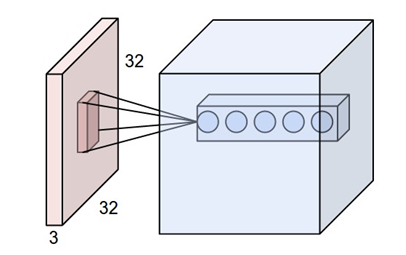
\includegraphics[width=0.6\textwidth]{./imgs/konvolucijski_sloj.png}
		\caption{Primjer ulazne slike 32x32x3 i rezultata izlaza nakon jednog konvolucijskog sloja dubine 5 \cite{CS231n}}
		\label{fg:konvolucijski_sloj}
	\end{center}
\end{figure}

Intuitivno konvolucijski slojevi će naučiti filtere koji će reagirati na određeni tip vizualnih svojstava, pa ima smisla dijeliti parametre filtera unutar svakog kanala neovisno o trenutno promatranom području slike.

Svaki filter ima onoliko pomičnih prozora koliko prethodni sloj ima kanala, a svaki pomični prozor ima prethodno određenu površinu receptivnog polja, npr. 3 prozora površine 3x3 kao u gornjem primjeru koji se pomiču po svom zaduženom kanalu. Moguće je svakom konvolucijskom filteru definirati korak (engl. stride) kojim se prozor pomiče po kanalima prethodnog sloja. Jedan položaj filtera daje jednu vrijednost u jednom izlaznom kanalu. Izlaz filtera je suma svih izlaza pojedinačnih prozora po kanalu (Slika \ref{fg:konvolucija}). Svaki prozor sa slike množi određenom težinom element na odgovarajućem mjestu te sumira dobivene vrijednosti svih prozora dobivajući vrijednost krajnjeg izlaza. Nakon izračuna svih vrijednosti sloja one se šalju u aktivacijsku funkciju i koriste se kao ulaz u sljedeće slojeve. 

\clearpage
\begin{figure}[!ht]
	\begin{center}
		\captionsetup{justification=centering}
		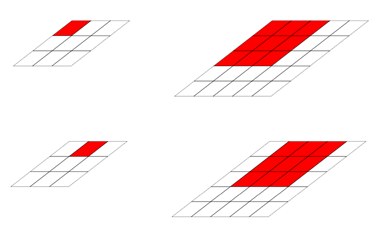
\includegraphics[width=0.6\textwidth]{./imgs/konvolucija.png}
		\caption{Primjer računanja izlaza (Lijevo) iz ulaza koji sadrži jedan kanal (Desno) pomicanjem prozora po kanalu \cite{DubokoUcenje}}
		\label{fg:konvolucija}
	\end{center}
\end{figure}

Korak pomaka (engl. stride) definira za koliko elemenata će se pomicati filter, odnosno svaki prozor pri računanju izlazne vrijednosti sljedećeg neurona. Veći korak utječe na dimenziju izlaznog sloja (Slika \ref{fg:pomak}).

\begin{figure}[!ht]
	\begin{center}
		\captionsetup{justification=centering}
		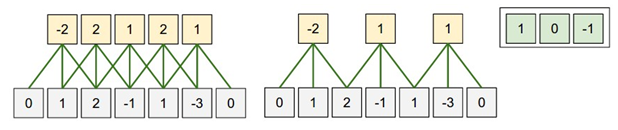
\includegraphics[width=0.6\textwidth]{./imgs/pomak.png}
		\caption{Utjecaj iznosa pomaka filtera na izlaze s prikazanim težinama na desnoj strani slike \cite{CS231n}}
		\label{fg:pomak}
	\end{center}
\end{figure}

Osim koraka pomaka, na dimenziju izlaza utječe i površina receptivnog polja filtera. Veće receptivno polje uzrokovat će manji broj izlaza jer će se na ulaznu sliku moći posložiti manja količina prozora iz kojih se računaju izlazne vrijednosti. Uobičajena praksa je proširiti ulaznu sliku dodavanjem nula (engl. padding) na rubove kako bi se nakon konvolucije zadržala dimenzija izlaza jednaka ulazu. Količina nula koje je potrebno dodati ovisi o receptivnom polju i koraku konvolucije.

Dodavanjem slojeva receptivno polje novih neurona se povećava ovisno o receptivnom polju prošlih neurona. Primjerice nakon dvije konvolucije s receptivnim poljem 3x3 i korakom jedan neuroni u drugom sloju vide veću površinu originalne slike od neurona u sloju prije njih (Slika \ref{fg:receptivno_polje}). Zbog toga dublji slojevi konvolucijske mreže uče prepoznavati složenije vizualne značajke poput kotača, dok niži slojevi uče prepoznavati jednostavne značajke poput rubova objekata. 

\begin{figure}[!ht]
	\begin{center}
		\captionsetup{justification=centering}
		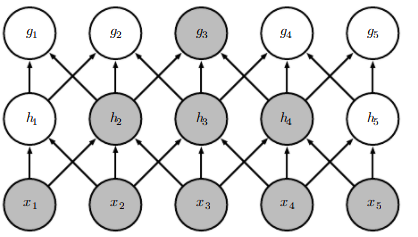
\includegraphics[width=0.6\textwidth]{./imgs/receptivno_polje.png}
		\caption{Povećanje receptivnog polja s dubinom mreže  \cite{deeplearningbook}}
		\label{fg:receptivno_polje}
	\end{center}
\end{figure}

\subsection{Slojevi sažimanja}

Sloj sažimanja je vrlo jednostavan, ali vrlo bitan dio konvolucijske mreže. Sažimanje obično računa neku statističke vrijednost nad receptivnim poljem poput maksimalne vrijednosti ili srednje vrijednosti. Ideja sloja sažimanja je smanjiti dimenzionalnost (Slika \ref{fg:sazimanje}) i broj potrebnih parametara mreže. Dodatni pozitivan efekt smanjena broja parametara je i smanjenje vjerojatnosti da se takva mreža prenauči na ulazne podatke.

Osim reduciranja dimenzionalnosti slojevi sažimanja unose invarijantnost na pomake u slici. Do intuitivnog objašnjenja prethodne tvrdnje možemo doći ako pretpostavimo da filter reagira na neki oblik u prethodnom sloju što prepoznajemo po većoj pozitivnoj vrijednosti izlaza od ostalih susjednih neurona (referenca na drugu sliku ispod). Budući da za klasifikaciju nije bitno znati gdje se oblik nalazi na slici nego nalazi li se na slici može se iskoristiti sažimanje maksimalnom vrijednosti. Takvo sažimanje će u sljedeće slojeve propustiti samo maksimalni odziv u promatranom prozoru (Slika \ref{fg:sazimanje2}).

\begin{figure}[H]
	\begin{center}
		\captionsetup{justification=centering}
		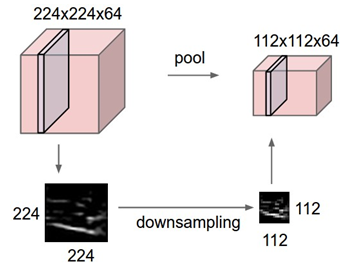
\includegraphics[width=0.6\textwidth]{./imgs/sazimanje.png}
		\caption{Sloj sažimanja s receptivnim poljem veličine 2x2 i pomakom 2 \cite{CS231n}}
		\label{fg:sazimanje}
	\end{center}
\end{figure}


\begin{figure}[H]
	\begin{center}
		\captionsetup{justification=centering}
		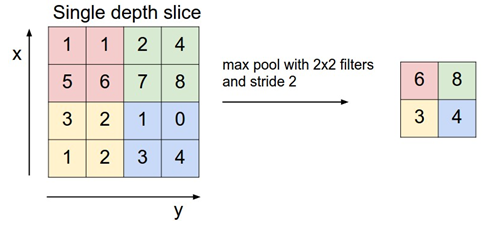
\includegraphics[width=0.6\textwidth]{./imgs/sazimanje2.png}
		\caption{Primjer sažimanja maksimalnom vrijednošću filterom 2x2 i pomakom 2 \cite{CS231n}}
		\label{fg:sazimanje2}
	\end{center}
\end{figure}

\subsection{Potpuno povezani slojevi}

Potpuno povezani slojevi dolaze iz najjednostavnijeg oblika neuronskih mreža, potpuno povezanih unaprijednih mreža, zbog čega će ovi slojevi biti objašnjeni direktno objašnjavanjem načina rada te vrste arhitekture mreža.
 
Potpuno povezana unaprijedna neuronska mreža je građena od slojeva koji se razlikuju jedino po aktivacijskoj funkciji na izlazu, ulazni sloj na koji stižu podaci čija je aktivacija funkcija identiteta, skrivenih slojeva na čijem se izlazu nalazi neka derivabilna nelinearna funkcija te izlaznog sloja s konačnim rezultatom izračuna s aktivacijom prikladnom za problem koji se nastoji riješiti (Slika \ref{fg:potpuno_povezana}). Svaki ulaz u neuron ima svoju težinu koja množi ulaz te se svi ulazi na kraju sumiraju i šalju u aktivacijsku funkciju. Rezultat aktivacijske funkcije zatim postaje ulaz u sljedeće slojeve ili predstavlja završni rezultat iz zadnjeg sloja.

\begin{figure}[!ht]
	\begin{center}
		\captionsetup{justification=centering}
		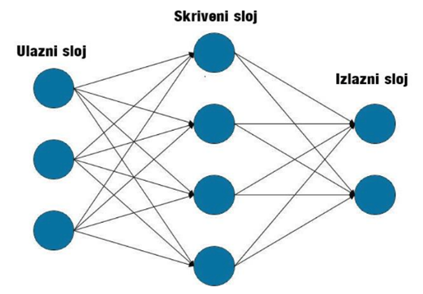
\includegraphics[width=0.6\textwidth]{./imgs/potpuno_povezana.png}
		\caption{Potpuno povezana unaprijedna neuronska mreža}
		\label{fg:potpuno_povezana}
	\end{center}
\end{figure}

\section{Analiza glavnih komponenti}

Analiza glavnih komponenti (engl. Principal component analysis - PCA) standardni je alat u modernoj analizi podataka - u različitim područjima od neuroznanosti do računalne grafike zbog toga što je jednostavna, neparametarska metoda za ekstrahiranje relevantnih informacija iz podatkovnog skupa \cite{PCA}.

Bez ulaženja u matematiku koja se može pronaći u radu \cite{PCA} PCA se može objasniti laičkim terminima kao tehnika koja pronalazi temeljne varijable koje najbolje diferenciraju podatkovni skup (poznatije kao glavne komponente - engl. principal components). Glavne komponente skupa su dimenzije po kojima je naš podatkovni skup najviše raspršen (Slika \ref{fg:pca_start}).

\begin{figure}[!ht]
	\begin{center}
		\captionsetup{justification=centering}
		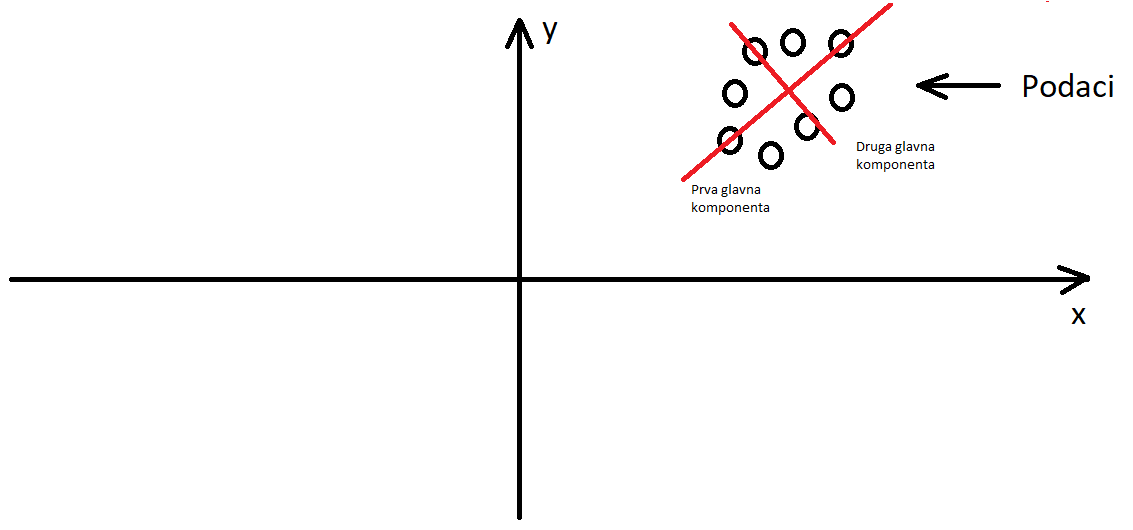
\includegraphics[width=0.6\textwidth]{./imgs/pca_start.png}
		\caption{Određivanje glavnih komponenti podatkovnog skupa}
		\label{fg:pca_start}
	\end{center}
\end{figure}

Nakon što je određen traženi broj glavnih komponenti (u slučaju sa slike njih dva) podatkovni skup se transformira u novi koordinatni sustav (Slika \ref{fg:pca_end}).

\begin{figure}[!ht]
	\begin{center}
		\captionsetup{justification=centering}
		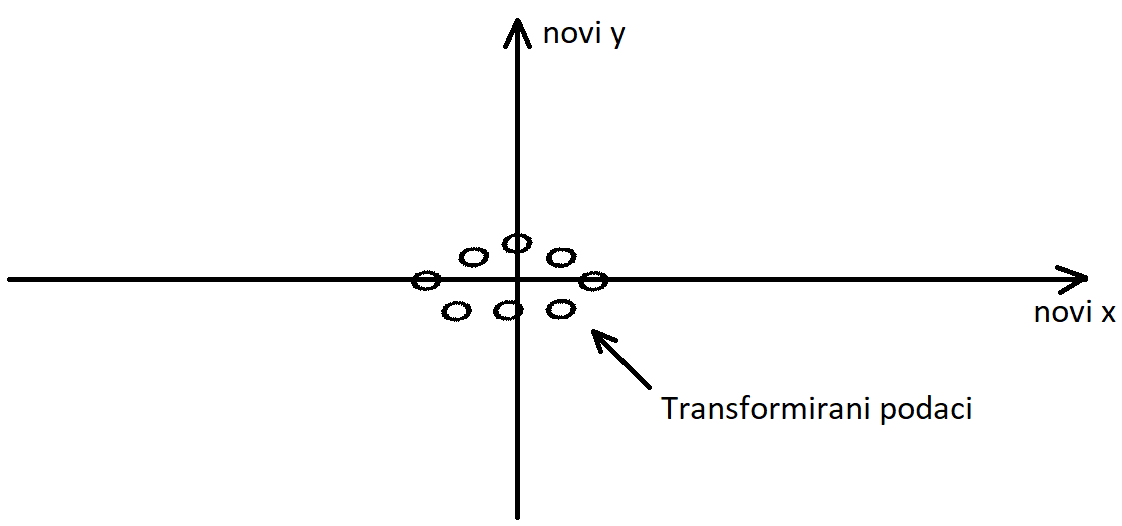
\includegraphics[width=0.6\textwidth]{./imgs/pca_end.png}
		\caption{Transformirani podatkovni skup}
		\label{fg:pca_end}
	\end{center}
\end{figure}

Iako se u gore navedenom primjeru dimenzionalnost podataka ne reducira (2D podaci ostaju u 2D prostoru) glavno područje primjene PCA tehnike je upravo redukcija dimenzionalnosti koja funkcionira na skoro identičan način. Razlikuje se po tome što se nakon određenih smjerova raspršenja oni poredaju silazno po svojstvenim vrijednostima te se odabere njih n (željena dimenzija na koju se reducira) nakon čega se podaci transformiraju u taj koordinatni prostor čime se gube ostale dimenzije s manjim svojstvenim vrijednostima. 

Važno je naglasiti da je glavna motivacija iza PCA tehnike uklanjanje korelacije u podatkovnom skupu odnosno uklonjanje zavisnosti drugog reda između podataka [3]. Način na koji PCA nastoji ostvariti taj cilj je pretpostavkom su glavne komponente međusobno ortogonalne zbog čega neće biti primjerena za podatkovne skupove poput onog na slici \ref{fg:pca_problem}.

\begin{figure}[!ht]
	\begin{center}
		\captionsetup{justification=centering}
		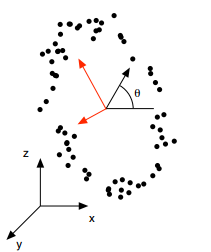
\includegraphics[width=0.6\textwidth]{./imgs/pca_problem.png}
		\caption{Podatkovni skup i crveno odabrane glavne komponente \cite{PCA}}
		\label{fg:pca_problem}
	\end{center}
\end{figure}


\section{VGG}

Arhitektura prvog isprobanog modela datira iz 2014., a dolazi sa sveučilišta Oxford čiji ju je tim koristio u ImageNet Large Scale Visual Recognition Challenge natjecanju. VGG tim, po kojem je mreža dobila i ime, ostvario je prvo mjesto iz zadatka lokalizacije objekata i drugo mjesto iz zadatka klasifikacije.

Njihov glavni doprinos je temeljita evaluacija arhitektura dubokih mreža koje koriste konvolucijske filtere malih dimenzija (3x3), čime su pokazali da se značajno poboljšanje u odnosu na tadašnje najbolje arhitekture može postići povećanjem dubine mreže na 16-19 slojeva dubine \cite{VGG}. 

Nakon evaluiranja više konfiguracija mreža VGG tim je pokazao su da dublja konvolucijska mreža nadmašuje rezultate mreža s manje slojeva, zbog čega smo u našim ispitivanjima koristili njihovu najdublju mrežu u stupcu E sa slike \ref{fg:vgg}.

\begin{figure}[!ht]
	\begin{center}
		\captionsetup{justification=centering}
		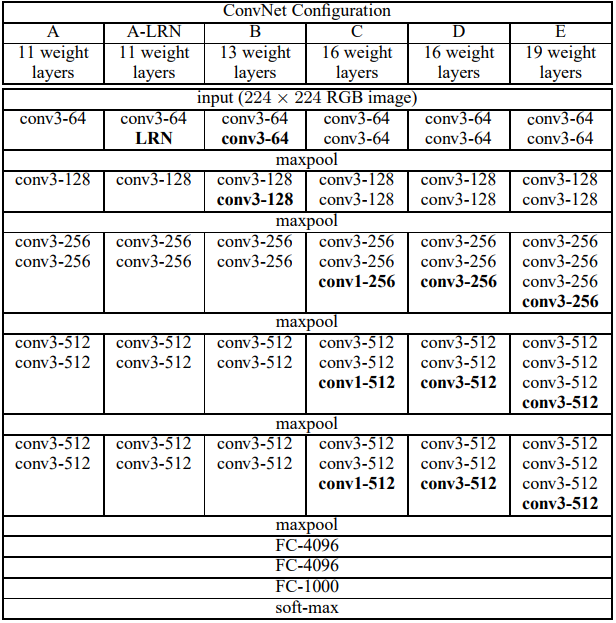
\includegraphics[width=0.6\textwidth]{./imgs/vgg.png}
		\caption{Konfiguracije VGG tima \cite{VGG}. Parametri konvolucije su prikazani kao conv<dimenzije filtera>-<broj kanala> a nakon svake se nalazi ReLU aktivacija koja nije prikazana}
		\label{fg:vgg}
	\end{center}
\end{figure}

\section{Inception v4}

Inception v4 model je Googleova četvrta iteracija Inception arhitekture koja se od VGG arhitekture najviše razlikuje po svojoj “širini”.  Arhitektura mreže u skraćenom prikazu Inception blokova se može vidjeti na slici (Slika \ref{fg:inceptionv4}). 

\begin{figure}[!ht]
	\begin{center}
		\captionsetup{justification=centering}
		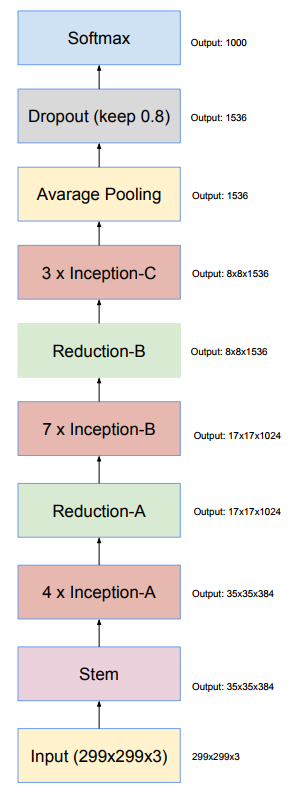
\includegraphics[width=0.4\textwidth]{./imgs/inceptionv4.png}
		\caption{Inception v4 \cite{Inceptionv4}}
		\label{fg:inceptionv4}
	\end{center}
\end{figure}

Inception blokovi su postali popularni nakon što je Googleova tadašnja arhitektura GoogLeNet izgrađena od Inception blokova ostvarila dobre performanse na natjecanju ImageNet. Intuitivno njihova glavna prednost je rješavanje problem odabira dimenzija filtera pri izgradnji mreže jer se sastoje od više grana konvolucija koje ulazni podatak obrađuju s različitim dimenzijama filtera. Zbog stablaste razgranatosti Inception blok iz ulaza može prepoznati kompliciranije uzorke jer svaka grana ulazni podatak promatra s različitim receptivnim poljem (npr. Slika \ref{fg:inception_blok_a}).
	
\begin{figure}[!ht]
	\begin{center}
		\captionsetup{justification=centering}
		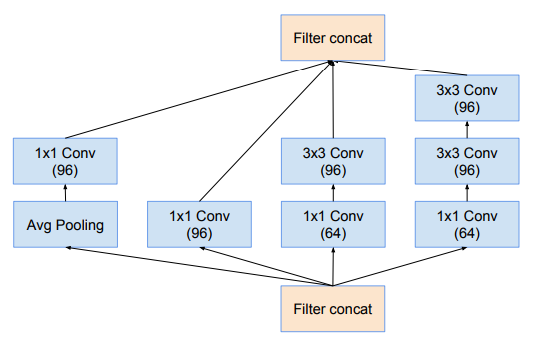
\includegraphics[width=0.6\textwidth]{./imgs/inception_blok_a.png}
		\caption{Inception-A blok  \cite{Inceptionv4}}
		\label{fg:inception_blok_a}
	\end{center}
\end{figure}

Inception moduli od kojih je građena mreža (A-C) obrađuju ulaze na sličan način. Zajednička karakteristika im je da izlazne dimenzije podatka ostanu jednake (npr. Inception-A na ulazu prima 35x35x384 a na izlazu daje 35x35x384), a razlikuju se po načinu obrade ulaznog podatka, točnije broja konvolucijskih slojeva u granama i njihovih parametara.

Osim Inception modula mreža se sastoji i od Reduction blokova koji su, uz ekstrakciju značajki, zaslužni za smanjivanje dimenzionalnosti ulaznog podatka. Kao i Inception blokovi razlika između Reduction bloka A i Reduction bloka B je samo u parametrima grana i dizajnu grana, a oba bloka smanjuju širinu i visinu ulaznog podatka za faktor 2 kombinacijom globalnog sažimanja ili konvolucija s korakom 2 (Slika \ref{fg:inception_reduction_a}).

\begin{figure}[!ht]
	\begin{center}
		\captionsetup{justification=centering}
		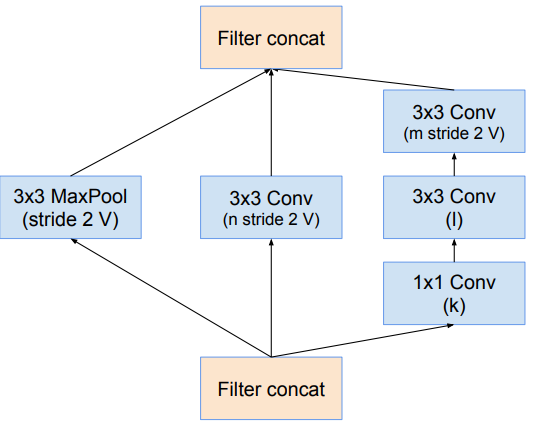
\includegraphics[width=0.6\textwidth]{./imgs/inception_reduction_a.png}
		\caption{Reduction-A blok (za Inception v4 k=192, l=224, m=256, n=384) \cite{Inceptionv4}}
		\label{fg:inception_reduction_a}
	\end{center}
\end{figure}
%%%%%%%%%%%%%%%%%%%%%%%%%%%%%%%%%%%%%%%%%%%%%%%%%%%%%%%%%%%%%%%%%%%%%%%%%%%%%%%%%%%%%%%
%% CHAPTER
\chapter{Rezultati i rasprava}

\section{Metrike sličnosti}

Prilikom uspoređivanja sličnosti vektora isprobali smo dvije metrike  euklidsku i kosinusnu udaljenost. 

Euklidska udaljenost definirana je kao L2 udaljenost između dva vektora (\ref{eq:euklidska_udaljenost}), a raspon vrijednosti iznosi od nula za točke koje se nalaze na istom mjestu u prostoru do beskonačnosti. Potencijalno negativna strana euklidske udaljenosti je zanemarivanje informacija o kutu između dvije točke. Primjer te situacije se može vidjeti na slici \ref{fg:euklidska_udaljenost} gdje su točka P, Q i R jednako udaljene od točke M, no kada bi uzimali informaciju o kutu u obzir najsličnija bi nam bila točka P.

\begin{equation}
\label{eq:euklidska_udaljenost}
EuclideanDistance(x,y) = \sqrt{\sum_{i=1}^n (x_i-y_i)^2}    
\end{equation}

\begin{figure}[!ht]
	\begin{center}
		\captionsetup{justification=centering}
		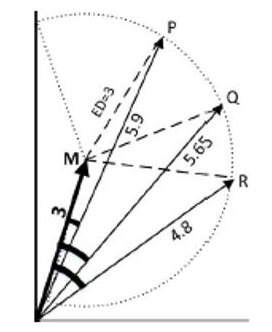
\includegraphics[width=0.3\textwidth]{./imgs/euklidska_udaljenost.png}
		\caption{Primjer euklidske udaljenosti \cite{VectorSimilarity}}
		\label{fg:euklidska_udaljenost}
	\end{center}
\end{figure}

Kosinusna udaljenost je definirana kao jedan - skalarni produkt dva vektora podijeljen s umnoškom njihovih normi (\ref{eq:kosinusna_udaljenost}), a raspon vrijednosti je od 2 za vektore koji gledaju u suprotnim smjerovima do 0 za kolinearne vektore. Potencijalno negativna strana kosinusne udaljenosti je zanemarivanje duljine vektora. Primjer se može vidjeti na \ref{fg:kosinusna_udaljenost} gdje su točke B, C i D jednako udaljene od točke A jer zatvaraju jednak kut, no kada bi se promatrala njihova euklidska udaljenost dobili bi različite rezultate.

\begin{equation}
\label{eq:kosinusna_udaljenost}
CosineDistance(x,y) = 1- cos(\pmb x, \pmb y) = 1 - \frac {\pmb x \cdot \pmb y}{||\pmb x|| \cdot ||\pmb y||}
\end{equation}

\begin{figure}[!ht]
	\begin{center}
		\captionsetup{justification=centering}
		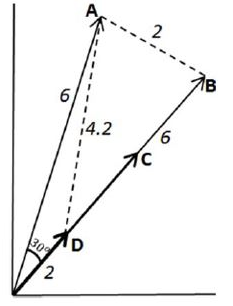
\includegraphics[width=0.3\textwidth]{./imgs/kosinusna_udaljenost.png}
		\caption{Primjer kosinusne udaljenosti \cite{VectorSimilarity}}
		\label{fg:kosinusna_udaljenost}
	\end{center}
\end{figure}

Obje metrike su davale skoro identične rezultate uz male promjene poretka između vraćenih slika. Jedan od razloga zašto smo dobili takve rezultate je velika dimenzionalnost prostora koji vektori razapinju. Posljedica toga je da dvije točke koje se nalaze blizu u prostoru ujedno zatvaraju i maleni kut zbog čega se smatraju sličnima u obje metrike.	

Nakon ispitivanja rezultata metrika odabrali smo kosinusnu udaljenost koja je davala zadovoljavajuće rezultate. Potencijalni problemi koji se mogu pojaviti kod te metrike u našem slučaju nisu pretjerano bitni budući da nam nije bitna duljina vektora već njegovo usmjerenje, odnosno relativan iznos aktivacija koje taj vektor opisuje. Primjerice ako našem sustavu predamo sliku mačke i tražimo ostale slične slike želimo vratiti sve vektore kojima su dominantni elementi koji detektiraju oči, njušku, uši mačke. Zbog toga nam je kosinusna udaljenost zadovoljavajuća jer vraća slike čiji reprezentativni vektori imaju jednake dominantne elemente unutar vektora.


\section{Predtrenirana arhitektura VGG}

VGG arhitektura je prva isprobana mreža za ekstrakciju značajki, točnije njen posljednji sloj konvolucijskog dijela mreže. Težinski koeficijenti mreže preuzeti su iz pobjedničke arhitekture ImageNet natjecanja čiji su filteri već naučeni prepoznavati komplicirane uzorke na ulaznim slikama.

Ulazna slika u mrežu je dimenzija 224x224x3, a finalni rezultat sloja kojeg koristimo je vektor od 25.000 elemenata. Budući da je krajnji cilj ostvariti reprezentaciju slike vektorom manjih dimenzija što bi omogućilo brže pretraživanje rezultat konvolucijske mreže se PCA modelom dalje reducira na 3000 dimenzija. Za treniranje PCA modela nasumično je izabrano 50.000 slika kako bi dobili što bolju procjenu glavnih komponenti.

Rezultati dobiveni na ovaj način za pojedine slike daju očekivane rezultate  (Slika \ref{fg:auti_vgg}), dok za druge već za top 5 najsličnijih slika pojedini rezultati budu ne povezani (Slika \ref{fg:greske_vgg}). 

\begin{figure}[!ht]
	\begin{center}
		\captionsetup{justification=centering}
		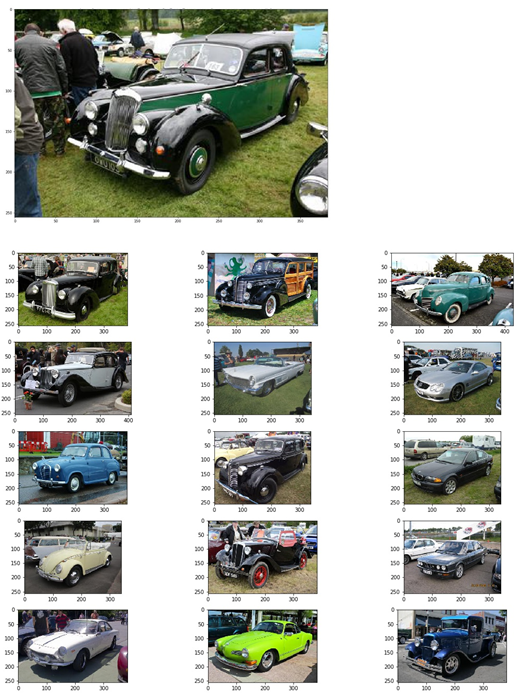
\includegraphics[width=0.8\textwidth]{./imgs/auti_vgg.png}
		\caption{Top 12 sličnih rezultata za sliku na vrhu}
		\label{fg:auti_vgg}
	\end{center}
\end{figure}

\begin{figure}[H]
\begin{center}
	\captionsetup{justification=centering}
	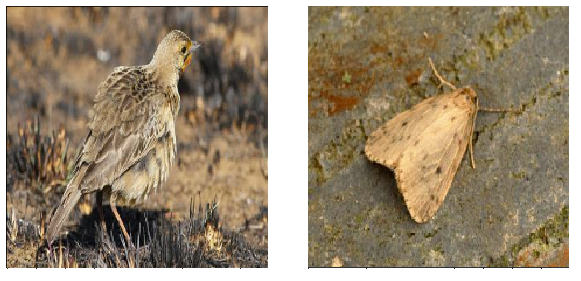
\includegraphics[width=0.8\textwidth]{./imgs/greske_vgg.png}
	\caption{Primjer slike čije se slične traže (lijevo) i slika u top 5 koja nije ispravna (desno)}
	\label{fg:greske_vgg}
\end{center}
\end{figure}

Dobri rezultati sažimanja, kao i lažni pozitivi dobiveni korištenjem jednostavnog VGG modela u daljnjim testiranjima koristili smo kao referencu koliko uspješno kompliciraniji modeli ekstrahiraju značajke iz ulazne slike.

\section{Predtrenirana arhitektura Inceptionv4}

Sljedeća arhitektura sa značajno većim kapacitetom je Inception v4. Kao i u slučaju arhitekture VGG i za Inception v4 smo preuzeli težinske koeficijente iz arhitekture naučene na skupu ImageNet.

Vođeni zaključcima koje smo dobili testirajući arhitekturu VGG za dohvaćanje sličnih slika prvi način ekstrakcije značajki, kao i u arhitekturi VGG, je bio uzimanjem izlaza zadnjeg sloja konvolucijske mreže. U ovom slučaju to je vektor od 1536 elemenata dobiven globalnim sažimanjem prosječnom vrijednošću. Dobivene vektore smo kasnije korištenjem PCA modela reducirali na 300 elemenata što je rezultiralo dosta lošim rezultatima unatoč velikom kapacitetu mreže (Slika \ref{fg:inception_zadnji_sloj_auti_greska}).

\begin{figure}[H]
	\begin{center}
		\captionsetup{justification=centering}
		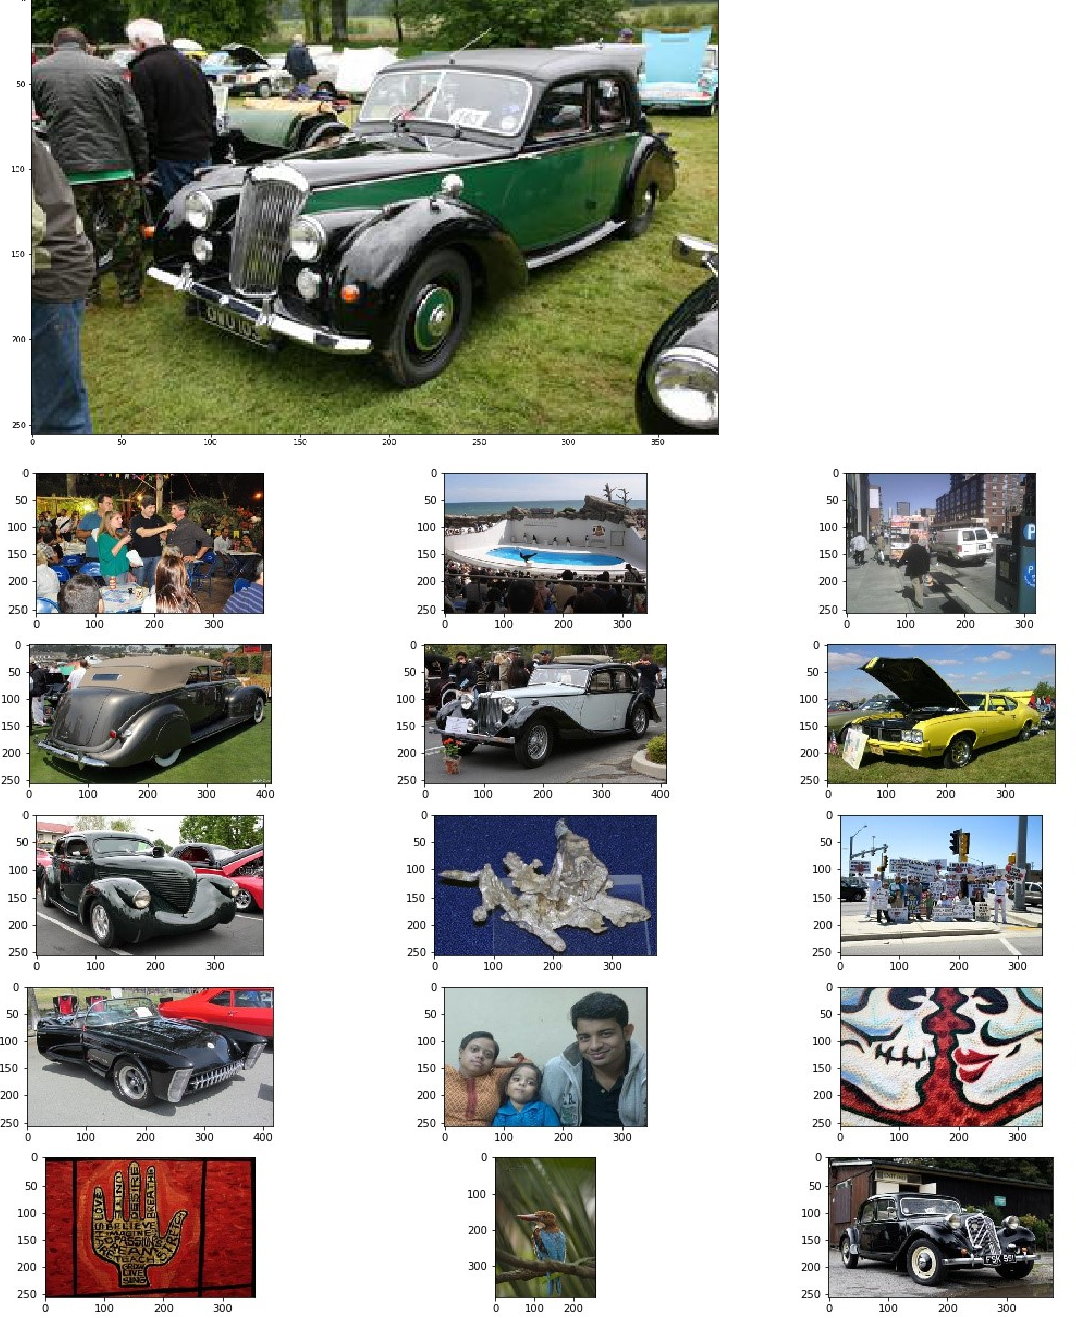
\includegraphics[width=0.8\textwidth]{./imgs/inception_zadnji_sloj_auti_greska.png}
		\caption{Top 12 sličnih rezultata za sliku na vrhu}
		\label{fg:inception_zadnji_sloj_auti_greska}
	\end{center}
\end{figure}

Razlog zašto redukcija predzadnjeg sloja dovodi do ovoliko loših rezultata djelomično se može objasniti time što mreža taj sloj koristi za završnu klasifikaciju i time nema neku semantičku interpretaciju. Budući da je krajnji cilj dobiti vektor koji se sastoji od 300 elemenata gdje je intenzitet svakog elementa u vektoru označava pojavljivanje određenog uzorka na ulaznoj slici vektor odlučili smo značajke ekstrahirati iz svih konvolucijskih slojeva mreže. 

Ekstrakcija značajki se vrši na sljedeći način, nad svakim konvolucijskim slojem u Inception mreži napravi se operacija globalnog sažimanja. Na primjer ako je izlaz konvolucijskog sloja 12 x 12 x 512 (visina, širina, broj kanala) globalnim sažimanjem svakog od kanala dobiti ćemo vektor 1x1x512. Dobiveni vektori svakog konvolucijskog sloja nakon globalnog sažimanja se izravnaju i konkateniraju u jedan veliki vektor s  \textasciitilde16000 elemenata.  Tako dobiveni elementi se zatim reduciraju na vektore od 300 elemenata korištenjem PCA modela. Kako bi nam rezultati bili što precizniji korišteni PCA model je prethodno istreniran korištenjem sto tisuća vektora od 16000 elemenata nasumično odabranih slika kako bi se što preciznije odredile glavne komponente podatkovnog skupa.

Primjer tako dobivenih rezultata može se vidjeti na sljedećim slikama \ref{fg:inception_globalno_sazimanje_auti}, \ref{fg:inception_globalno_sazimanje_ptice}, \ref{fg:inception_globalno_sazimanje_ptice}, a korišteni kod za generiranje i dodatne rezultate moguće je vidjeti na \cite{AVSP}.

\begin{figure}[H]
	\begin{center}
		\captionsetup{justification=centering}
		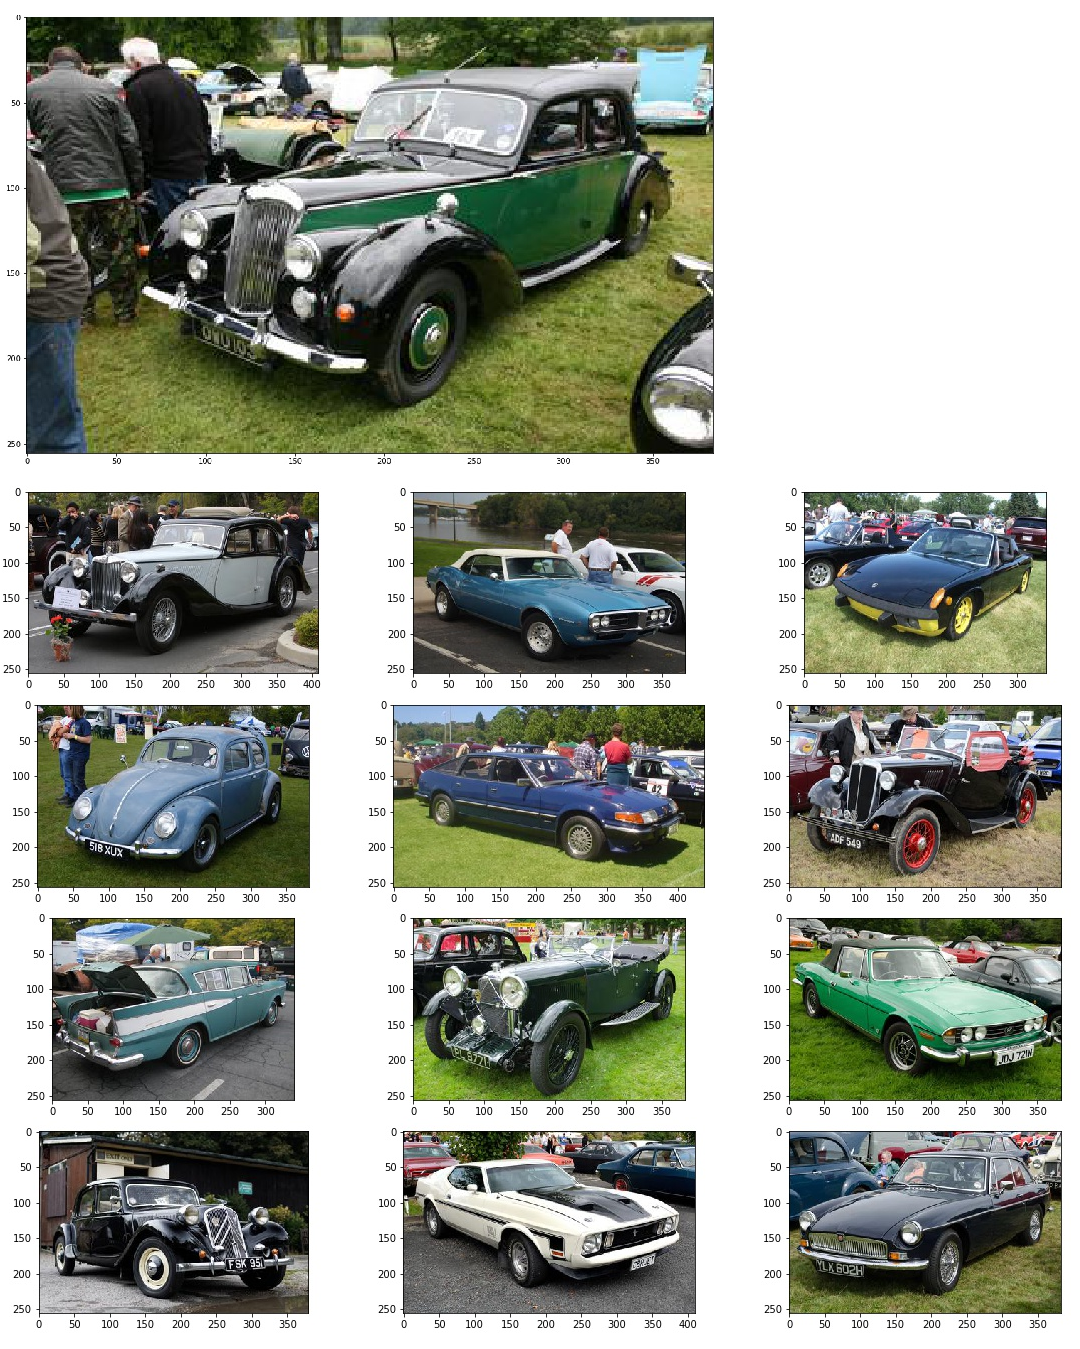
\includegraphics[width=0.8\textwidth]{./imgs/inception_globalno_sazimanje_auti.png}
		\caption{Top 12 sličnih rezultata za sliku na vrhu}
		\label{fg:inception_globalno_sazimanje_auti}
	\end{center}
\end{figure}

\begin{figure}[H]
	\begin{center}
		\captionsetup{justification=centering}
		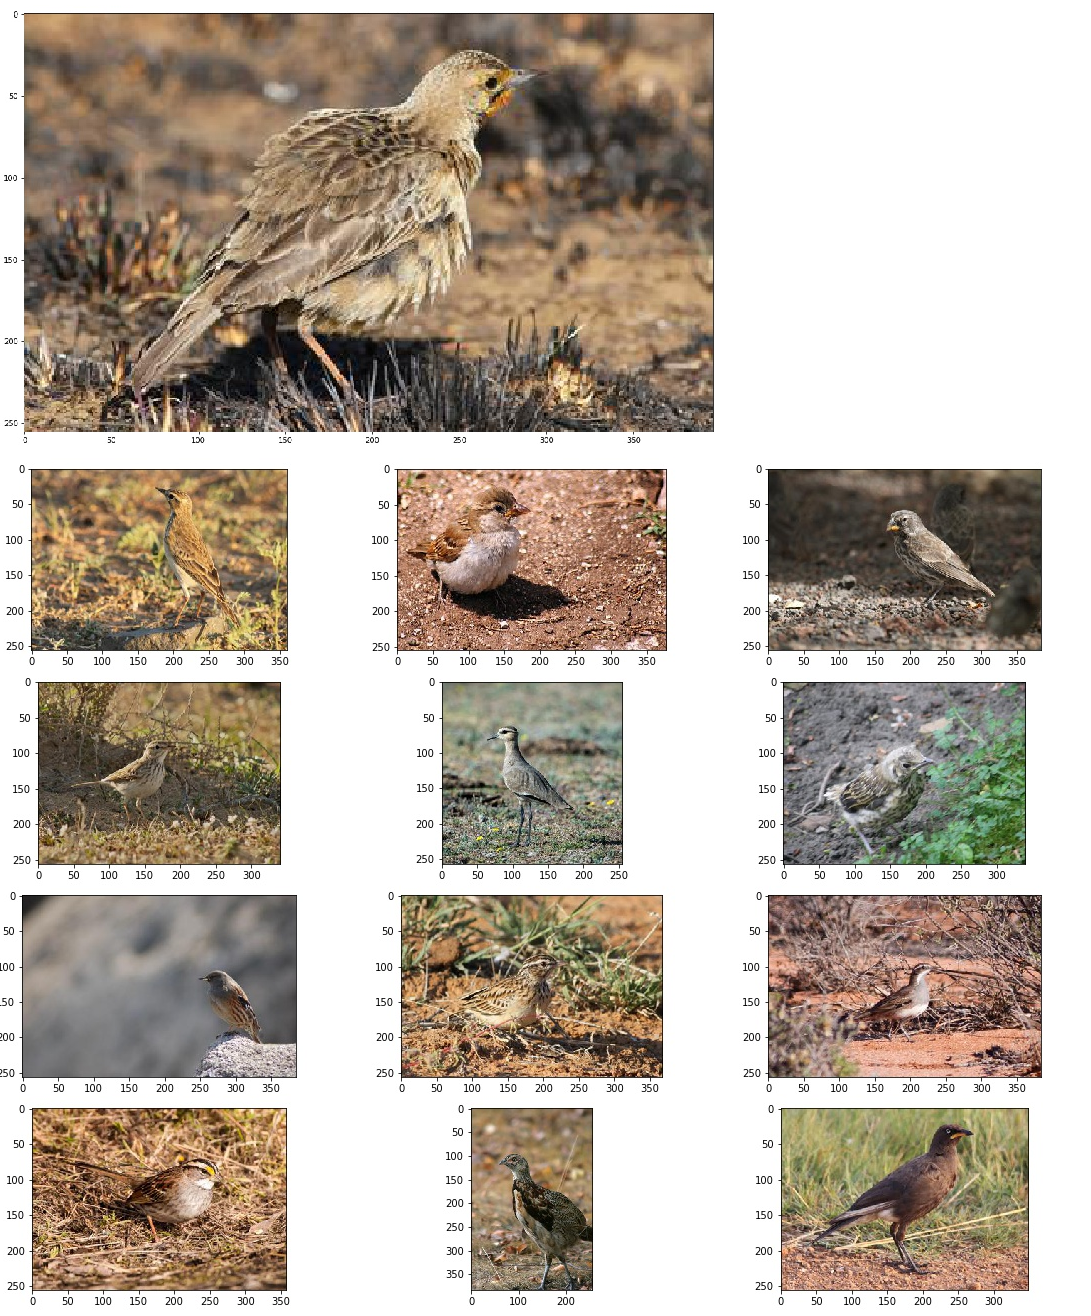
\includegraphics[width=0.8\textwidth]{./imgs/inception_globalno_sazimanje_ptice.png}
		\caption{Top 12 sličnih rezultata za sliku na vrhu}
		\label{fg:inception_globalno_sazimanje_ptice}
	\end{center}
\end{figure}


\begin{figure}[H]
	\begin{center}
		\captionsetup{justification=centering}
		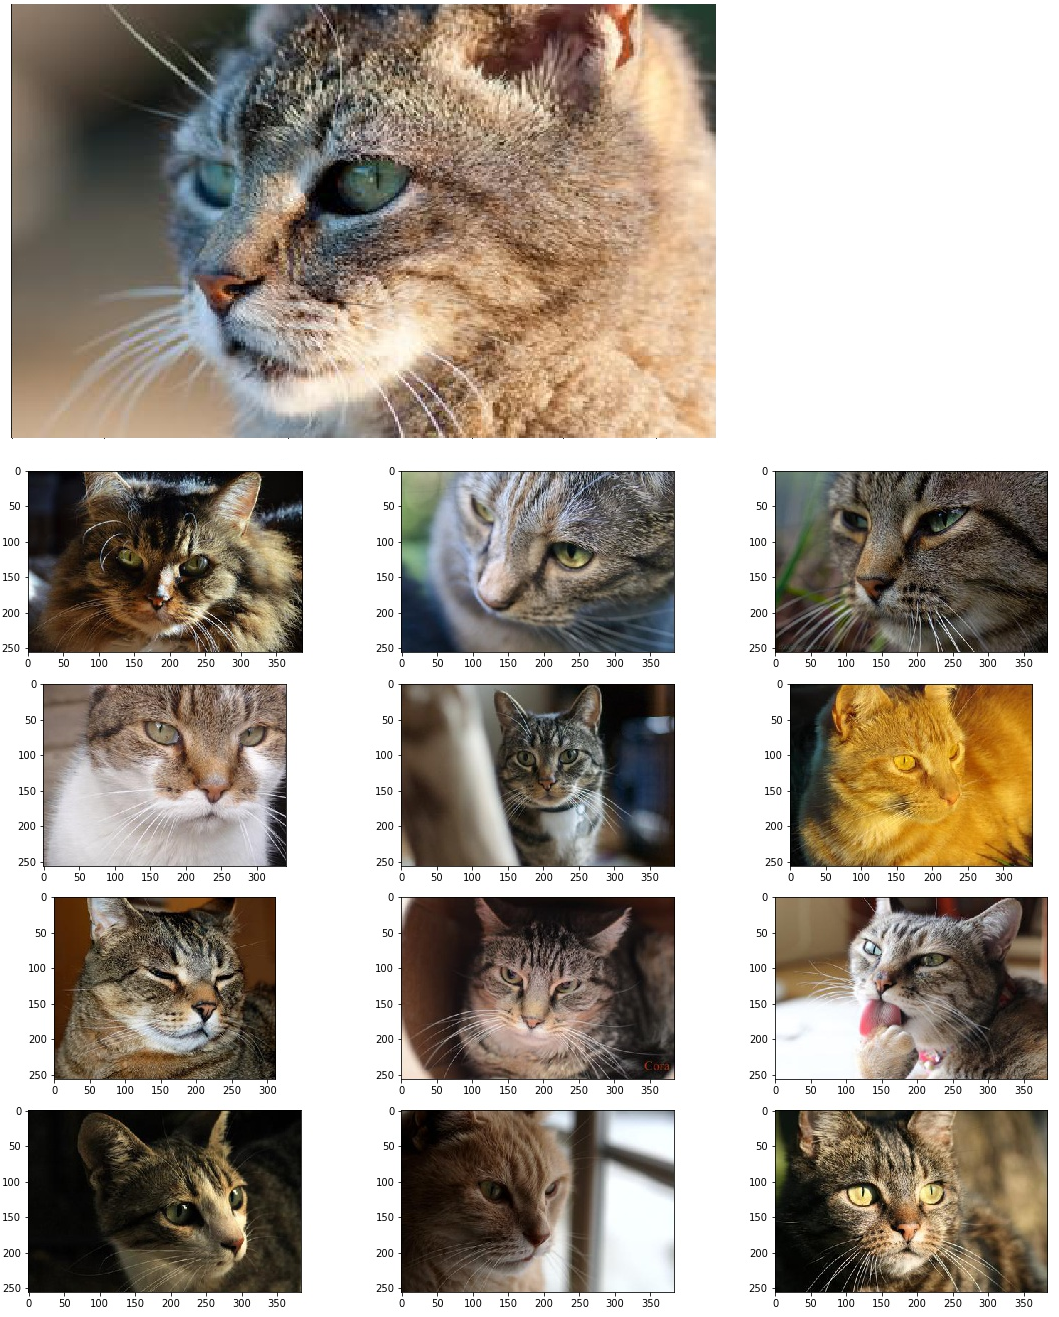
\includegraphics[width=0.8\textwidth]{./imgs/inception_globalno_sazimanje_macke.png}
		\caption{Top 12 sličnih rezultata za sliku na vrhu}
		\label{fg:inception_globalno_sazimanje_macke}
	\end{center}
\end{figure}

Kao što se vidi iz prikazanih slika unatoč reprezentiranja slike sa svega 300 elemenata što predstavlja višestruku uštedu prostora (\ref{tbl:usteda_prostora}) vektor i dalje dobro ekstrahira suštinu slike te slične slike grupira u bliske nakupine što je posebno vidljivo u sljedećem poglavlju.


\begin{table}[htb]
	\caption{Primjer uštede prostora}
	\label{tbl:usteda_prostora}
	\centering
	
	\begin{tabular}{lcc| c}
		\toprule
		{} & \thead{Dimenzije slike} & \thead{Ukupno elemenata} & \thead{Faktor uštede} \\
		\midrule
		\textit{{480p (12:9)}} & 640x480 & 921 600 & 307 200\%\\
		\textit{720p Widescreen} & 1280x720 &  2 764 800 & 921 600\%  \\		
		\textit{1080p HD Widescreen} & 1920x1080 &  6 220 800 & 2 073 600\%  \\
		
		\bottomrule
	\end{tabular}
\end{table}

\section{T-SNE prikaz smanjenog skupa podataka}

Budući da korišteni podskup slika Googleov OpenImage \cite{openimages} podatkovnog skupa velik (\textasciitilde1 milijun slika) i anotacije klasa nisu nužno točne jer ih je većina generirana automatskom strojnom anotacijom korištenjem servisa poput Google Cloud Vision API za vizualizaciju smo odabrali manji skup podataka koji je anotiran ručno.

Odabrani skup podataka je STL-10 \cite{STL10} čije slike imaju dimenziju 96x96x3, a nastao je po uzoru na podatkovni skup CIFAR-10 koji se obično koristi za vrednovanje modela.

Korištenjem metode t-SNE, značajke dobivene iz najboljeg modela Inception v4 s globalnim sažimanjem kanala su prikazane u 2D prostoru. Na slici \ref{fg:stl_10_tsne} se vidi da su podaci grupirani u nakupine uz poneka miješanja grupa poput slika jelena i konja. Razlog tome može biti zbog vrlo slične pozadine slike i kuta snimanja gdje se značajke jelena (rogovi) ne vide jasno na slici zbog čega ih mreža lako može zamijeniti jer su obje životinje približno jednake boje.

Moguće je dodatno poboljšati performance mreže za određivanje sličnosti tako da se radi redukcija dimenzionalnosti modelom PCA na značajkama dobivenim iz klasa koje želimo preciznije razlikovati, u ovome slučaju klasa iz STL-10 podatkovnog skupa.

\begin{figure}[!ht]
	\begin{center}
		\captionsetup{justification=centering}
		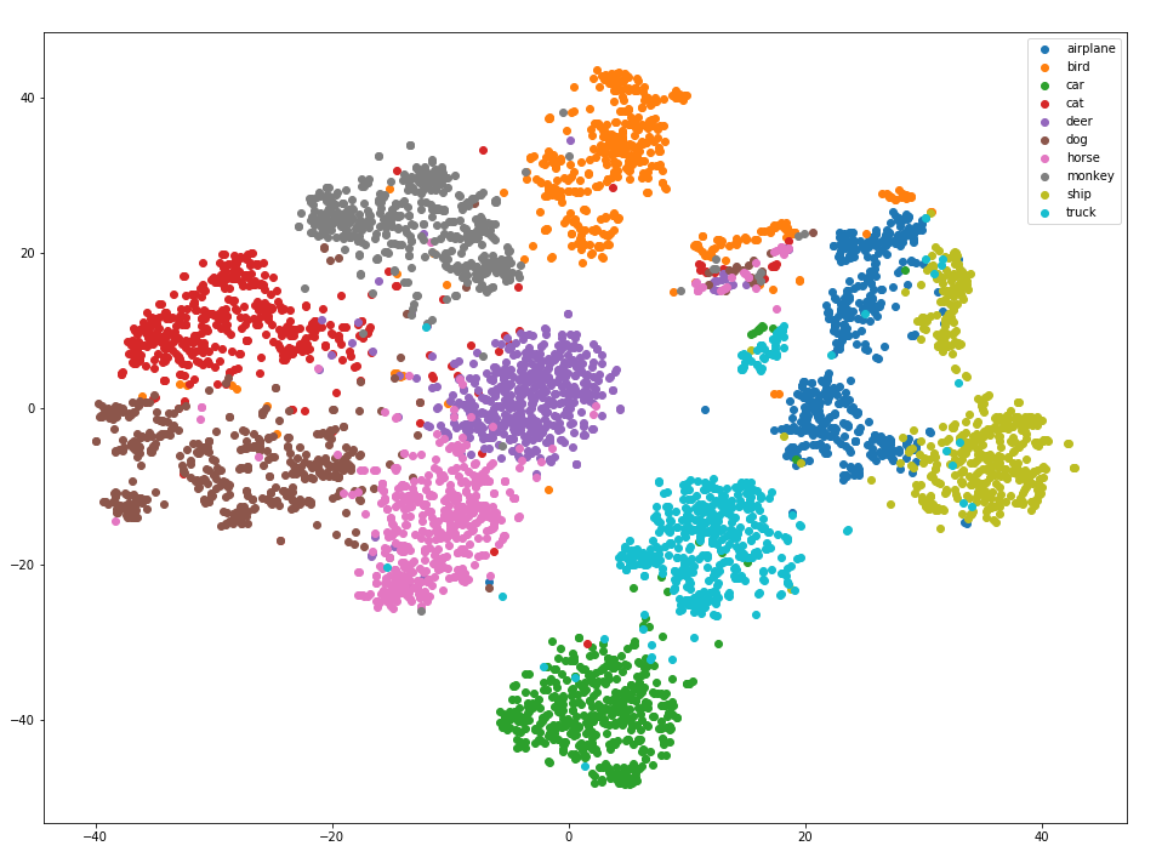
\includegraphics[width=1.\textwidth]{./imgs/stl_10_tsne.png}
		\caption{STL-10 dataset reprezentativni vektori prikazani u dvije dimenzije}
		\label{fg:stl_10_tsne}
	\end{center}
\end{figure}

%%%%%%%%%%%%%%%%%%%%%%%%%%%%%%%%%%%%%%%%%%%%%%%%%%%%%%%%%%%%%%%%%%%%%%%%%%%%%%%%%%%%%%%
%% CHAPTER
\chapter{Demo preporučitelj po sadržaju}

\section{Neki tvoj section?}


%%%%%%%%%%%%%%%%%%%%%%%%%%%%%%%%%%%%%%%%%%%%%%%%%%%%%%%%%%%%%%%%%%%%%%%%%%%%%%%%%%%%%%%
%% CHAPTER
\chapter{Zaključak}

Rezultati su pokazali da je korištenjem dubokih modela moguće značajno reducirati reprezentaciju slika na nisko dimenzionalan vektor koji čuva njenu semantiku. Takva redukcija ostvaruje veliku uštedu korištene radne memorije i zbog svoje male dimenzionalnosti omogućuje brzu usporedbu i dohvat sličnih slika preko njihovih reduciranih reprezentacija. 

Budući da je u okviru ovog istraživanja korišten veliki i raznoliki skup podataka, kao i duboki modeli koji su trenirani na skupu podataka s drugačijom distribucijom od onoga na kojem je testiran to ostavlja prostor za dodatne eksperimente i naši rezultati određuju donju granicu performansi sustava. Razumno je pretpostaviti da bi se dodatna poboljšanja postigla kada bi se duboki model korišten za redukciju istrenirao na skupu podataka s istom distribucijom kao podaci koji će se koristiti u sustavu preporuke. Tako istrenirani model omogućio bi izbor manje dimenzije reprezentativnog vektora čime bi se ostvarile još bolje performanse sustava u vidu preciznosti i memorijskih/vremenskih zahtjeva pretrage.

Daljnja istraživanja, kao i napreci u području dubokog učenja ostavljaju mnogo prostora za detaljnije istraživanje dodatnih mogućnosti ekstrahiranja značajki.

%%%%%%%%%%%%%%%%%%%%%%%%%%%%%%%%%%%%%%%%%%%%%%%%%%%%%%%%%%%%%%%%%%%%%%%%%%%%%%%%%%%%%%%
%% CHAPTER
\chapter{Sažetak}

%%%%%%%%%%%%%%%%%%%%%%%%%%%%%%%%%%%%%%%%%%%%%%%%%%%%%%%%%%%%%%%%%%%%%%%%%%%%%%%%%%%%%%%

%%%%%%%%%%%%%%%%%%%%%%%%%%%%%%%%%%%%%%%%%%%%%%%%%%%%%%%%%%%%%%%%%%%%%%%%%%%%%%%%%%%%%%%
%% CHAPTER
\chapter{Summary}

%%%%%%%%%%%%%%%%%%%%%%%%%%%%%%%%%%%%%%%%%%%%%%%%%%%%%%%%%%%%%%%%%%%%%%%%%%%%%%%%%%%%%%%
%% DONE
\bibliography{references}
\bibliographystyle{unsrtnat}
\pagebreak
\begin{sazetak}
	sažetak
	
	\kljucnerijeci{ključne riječi}
\end{sazetak}

\engtitle{Extracting Image Features Using Deep Learning for Better Image Recommendation System Performance }
\begin{abstract}
	description
	
	\keywords{keywords}
\end{abstract}
\end{document}